\documentclass[../main.tex]{subfiles}
\begin{document}
	\textbf{Напоминание: } $\A$ нормальный оператор $\Space \A \A^* = \A^* \A \n 
	\slide{100px} \forall x, y \in V \Space  (\A x, \A y) = (\A^* x, \A^* y)$
	\begin{theorem}[Канонический вид матрицы нормального оператора в унитарном пространстве]\ \n
		$\A \in End(V), (V (\cdot, \cdot))$ \underline{унитарное пространство}\\
		$\A$ нормальный оператор $\Leftrightarrow \exists$ \underline{о.н.б.} $V$ такой, что матрица оператора $\A$ в этом базисе будет иметь диагональный вид.\n 
		$\Lambda = diag(\lambda_1 \ldots \lambda_n) = \begin{pmatrix}
		\lambda_1 & & 0\\
		& \ddots & \\
		0 & & \lambda_n
		\end{pmatrix} , \Space \lambda_i \in \mathbb C$, при этом \n 
		матрица оператора $\A^*$, очевидно, также будет иметь диагональный вид \n $\vec \Lambda = diag (\vec{\lambda_1}, \ldots \vec{\lambda_n}) = \begin{pmatrix}
			\vec{\lambda_1} & & 0 \\
			& \ddots\\0 & & \vec{\lambda_n}
		\end{pmatrix}$
	\end{theorem}
	\begin{remark}
		\ \begin{mylist}
			\item Очевидно, что о.н.б. состоит из с.в. (попарно-ортог. и нрмиров.) \\
			$\lambda$ соотв. с.ч.
			\item $\forall $ нормальный оператор в унитарном пр-ве является о.п.с. Обратное, вообще говоря, неверно. Не всякий о.п.с. имеет именно \underline{о.н.б.}, в котором матрица опер. диагона.
		\end{mylist}
	\end{remark}
	\begin{proof}\ \\
		$(\Leftarrow)$ очевидно, в о.н.б. $\begin{matrix}
			A^{\circled *} = A^* = \vec{A^T} = \vec{\Lambda^T} = diag (\vec \lambda_1 \ldots \vec \lambda_n) \\
			A^{\circled *} = A A^{\circled *} \Rightarrow \A \text{ нормальный оператор}
		\end{matrix}$\n 
		$(\Rightarrow) \Space v_1 $ с.в. $\A$ соотв. с.ч. $\lambda_1 \Rightarrow v_1$ с.в. $\A^*$ с.ч. $\vec \lambda_1\n 
		L := span(v_1)$ инвариант. отн-но $\A$ и $\A^* \Rightarrow L^\perp$ инвар. отн-но $\A$ и $\A^* \n 
		\Rightarrow \A|_{L^\perp}$ и $\A^*|_{L^\perp}$ останутся взаимно-сопряж. и нормальн.\n
		\textbf{Докажем м.м.и.:} (по $dim V = n$)\
		\begin{mylist}
			\item \underline{база:} $n = 1$ утв. очев.
			\item \underline{инд. предпол.} $\pu$ верно для $n=k$
			\item \underline{инд. переход} докаэем что тогда верно $n = k+1 ?\n 
			L = span(v_1) \Space V = L \oplus L^\perp \Space dim L^\perp = k \Rightarrow$ по инд. предпол. \n 
			($\A|_{L^\perp}$ и $\A^*|_{L^\perp}$ тоже нормальные) $\Space \exists$ о.н.б. $v_2, v_3, \ldots, v_{k+1}$ т.ч.\n матрица $\A$ будет иметь вид $diag(\lambda_1 \ldots \lambda_{k+1})$, \\
			а матрица $\A^*$ -- $diag(\vec \lambda_2 \ldots \vec \lambda_{k+1})\n 
			L\oplus L^\perp = V = span(\underset{\text{попарно ортог. и нормир.}}{v_1, v_2, \ldots, v_{k+1}}) \Space \A v_1 = \lambda_1 v_1 \n 
			\Rightarrow$ матрица будет иметь блочно-диагональный вид\n 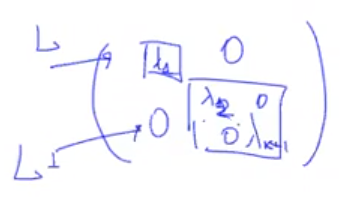
\includegraphics[width=150px]{pic105} $\begin{matrix}
				= \Lambda = diag(\lambda_1 \lambda_2 \ldots \lambda_{k+1})\\
				A^{\circled *} = \vec{A^T} = \vec \Lambda
			\end{matrix}$
		\end{mylist}
	\end{proof}
	\begin{corollary}\ \\
		$\A$ нормальный оператор в \underline{унитарном} пр-ве $V \Leftrightarrow V = \bigoplus\limits_{\stackrel{\lambda}{\text{с.ч.}}} V_\lambda \text{ собств. подпр.} \Space \underset{\lambda\neq \mu}{V_\lambda \perp V_\mu}$
	\end{corollary}
	\begin{proof}
		Очевидно из теоремы.
	\end{proof}
	\begin{corollary}
		$A_{n\times n} \; \; a_{ij} \in \mathbb C \Space A^* = \vec{A^T}\n 
		\forall$ \underline{норм.} матрицы $A \; (A A^* = A^* A) \; \exists$ \underline{унитарн.} матрица $T \; (T^* = T^{-1})$, \n 
		т.ч. $\boxed{T^{-1} A T = \vec{T^T} A T = \Lambda = diag(\lambda_1 \ldots \lambda_n)}$, где $\lambda_i$ с.ч. матрицы $A$
	\end{corollary}
	\begin{proof}\belowbaseline[-14pt]{
			$
			\begin{matrix}
				A \text{ в канонич. } \overset{e}{\text{базисе }} \mathbb C^n \\
				A^{\circled *} = A^* = \vec{A^T} \\ 
				\text{матрица соотв. } \A^*
			\end{matrix}
		$
		} -- матрица оператора $\A \n 
		A^* A = A A^* \Rightarrow \A$ нормальн. $\Rightarrow$ применяем теорему \n 
		$\exists$ о.н.б. $v_1 \ldots v_n \leadsto T = T_{e\rightarrow v} \\ $
		т.к. о.н.б. $\vec{T^T} = T^* = T^{-1}$, т.е. $T$ \underline{унитарн.} $\Rightarrow$ по формуле преобр. матрицы в новом базисе \n
		$\slide{200px} A' = T^{-1} A T = \underbracket{\vec{T^T}}_{T^*} A T = \Lambda = diag(\lambda_1 \ldots \lambda_n)$
	\end{proof}
	$\pu V(\cdot, \cdot)$ \underline{евклидово про-во} \n 
	не все корни хар. мн-на вещ. $\Rightarrow$ не все корни это с.ч. оператора \n 
	(\underline{см. 7.6}) \Space $V_\mathbb C$ -- комплексификация $V$ \belowbaseline[-14pt]{
		$\begin{matrix}
			\forall x, y \in V \leftrightarrow z = x + i y \in V_\mathbb C \\
			e_1 \ldots e_n \text{ базис } V \rightarrow e_1 \ldots e_n \; \text{ базис }V_\mathbb C \\
			v_1 \ldots v_k \text{ лин. нез. }\Leftrightarrow \vec v_1 \ldots \vec v_k \text{ лин. нез. }\\
			\vec z = x - iy
		\end{matrix}$
	}
	\begin{defin}
		Определим скалярное (псевдоскал.) пр-ве на $V_\mathbb C: \n 
		\begin{matrix}
			\forall x, y \in V \Space (\leftrightarrow z = x + i y) \\
			\forall u, v \in V \Space (\leftrightarrow \omega = u + i v)
		\end{matrix} \Space (z, \omega) = (x + iy, u + i v) \overset{def}{=} (x, u) + (y, v) + i((y, u) - (x, v))$
	\end{defin}
	\underline{Упр}.:  удовлетворить 1-4 свойства псевдоскал. пр-я $(V_\mathbb C, (\cdot, \cdot))$ \underline{унит. пр-во} \n 
	\underline{Упр}.:  $\vec{(z_1, z_2)} = (\vec z_1 , \vec z_2) \Space \forall z_1, z_2 \in V_\mathbb C$\n 
	$\A \in End(V) \Sspace \A_\mathbb C \in End(V)$ \Space \underline{продолжение вещ. опер.} $\A$ на $V_\mathbb C$ \\
	\begin{minipage}[t]{0.3\textwidth}
		$\forall x + i y \in V_\mathbb C \n x, y \in V$
	\end{minipage} \begin{minipage}[t]{0.6\textwidth}
		$\A_\mathbb C(x + i y) = \A x + i \A y \n 
		e_1 \ldots e_n$ базис $V \leadsto e_1 \ldots e_n$ базис $V_\mathbb C \n 
		\A \leftrightarrow A_{\text{вещ.}} \Sspace \A_\mathbb C \leftrightarrow A_{\text{вещ.}}$
	\end{minipage}
	\begin{stat}
		$\boxed{(\A_\mathbb C)^* = (\A^*)_\mathbb C}$
	\end{stat}
	\begin{proof}
		$e_1 \ldots e_n$ о.н.б. $V \Rightarrow e_1 \ldots e_n$ базис $V_\mathbb C \n 
		(e_k, e_j)_\mathbb C = (e_k + i \cdot \0 , e_j + i\cdot \0) = (e_k, e_j) = \delta_{kj} \Rightarrow$ о.н.б. в $V_\mathbb C$ \n 
		\begin{minipage}[t]{0.3\textwidth}
			в $V:$ \n 
			$\A \leftrightarrow A\\ 
			\A^* \leftrightarrow A^T = A^*$
		\end{minipage}
		\begin{minipage}[t]{0.6\textwidth}
			в $V_\mathbb C: $ \n 
			$\A_\mathbb C \leftrightarrow A \\ 
			(\A^*)_\mathbb C \leftrightarrow A^* = A^T$
		\end{minipage}\n 
	$\A_\mathbb C \leftrightarrow A$ в о.н.б. $V_\mathbb C \Rightarrow (\A_\mathbb C)^* \leftrightarrow \underset{\text{вещ.}}{\vec{A^T}} = A^T = A^* \n 
	\Rightarrow$ матрицы операторов $(\A_\mathbb C)^*$ и $(\A^*)_\mathbb C$ совпадают в о.н.б. $\Rightarrow \n \Rightarrow$ совпадают в любом базисе $\Rightarrow (\A_\mathbb C)^* = (\A^*)_\mathbb C$
	\end{proof}
	\textbf{Следствие:}
		$\A$ норм. опер. в евклид. $V \Rightarrow \A_\mathbb C$ норм. опер. в $V_\mathbb C$ (очевидно).
	\begin{theorem}[\underline{Канонический} вид матрицы \underline{нормального} оператора в \underline{евклидовом} пр-ве]\ \\
		$\A \in End(V), (V, (\cdot, \cdot))$ \underline{евкл. пр-во} \n 
		$\A$ норм. опер. $\Leftrightarrow \exists$ о.н.б. $V$ такой, что матрица оператора $\A$ в этом базисе будет иметь блочно-диагональный вид: \n 
		$\Lambda = \begin{pmatrix}
			\begin{pmatrix}
				\lambda_1 & & 0 \\
				& \ddots \\
				0 & & \lambda_k
			\end{pmatrix} & & &  0\\
			& \begin{pmatrix}
				\Phi_1\end{pmatrix} \\
				& & \ddots\\
				0 & & & \begin{pmatrix}
					\Phi_m
				\end{pmatrix}
		\end{pmatrix}$, где \Space $\begin{matrix}
			\lambda_s \in \R \n 
			\Phi_j = \begin{pmatrix}
				\alpha_j & \beta_j \\
				-\beta_j & \alpha_j
			\end{pmatrix} & \alpha_j, \beta_j \in \R
		\end{matrix} $\n 
		При этом матрица оператора $\A^*$, очевидно, также будет иметь блочно-диаг. вид: $\Lambda^T$
	\end{theorem}
	\begin{remark}
		Очевидно, $\lambda_1 \ldots \lambda_k$ собств. ч. $\A$  и первые $k$ векторов базиса -- это о. н. с. в.
	\end{remark}
	\begin{proof}
		$(\Leftarrow) \n \begin{matrix}
			\begin{matrix}
				\Lambda \Lambda^T = \Lambda^T \Lambda \text{ (упр.)}\\
				\Updownarrow\\
				A A^* = A^* A
			\end{matrix} & \text{ о.н.б. } A^{\circled *} = A^* = A^T \text{ т.к. евкл.} & \Sspace \Rightarrow \A \text{ норм. опер.}
		\end{matrix}$\n \\
		$(\Rightarrow) \Space \A$ норм. опер. $\rightarrow \underset{\text{норм. опер.}}{\A_\mathbb C}$ продолж. $\A$ на $V_\mathbb C \underset{\text{сле-вие 1}}{\Leftrightarrow} V_\mathbb C = \underset{\begin{matrix}
				\lambda \text{ с.ч. } \A_\mathbb C \\
				\text{т.е. все корни}\\
				\chi_{A_\mathbb C}
			\end{matrix}}{\bigoplus V_\lambda} \Space \underset{\lambda \neq \mu}{V_\lambda \perp V_\mu}\n 
		\chi_\A(t) = \chi_{\A_\mathbb C}(t) $ \Space (см. 7.6) \\
		\begin{mylist}
			\item $\underset{\lambda \text{ с.ч.} \A \Space u \text{ -- с.в.}}{\lambda \in \R \text{ корень } \chi_\A \Space} (\chi_\A(\lambda) = 0) \Rightarrow \lambda$ с.ч. $\A_\mathbb C$ с.в. $\omega = \underset{\mathlarger{u, v \text{ с.в. для } \A \; (u, v \in Ker (\A -\lambda \E))}}{u + i v \Space \circled{?}}\n 
			\A_\mathbb C \omega = \A u + i \A v = \lambda u + i \lambda v = \lambda (u + i v) = \lambda \omega \n 
			\underset{\text{для } \A_\mathbb C}{V_\lambda} = (Ker (\A - \lambda \E))_\mathbb C \Sspace $\belowbaseline[-14pt]{
			$\begin{matrix}
				V_\lambda = \underset{\stackrel{\uparrow}{\mathbb C}}{span}(v_1 \ldots v_k) \Space v_j \text{ попарно-орт. и норм.}\n 
				Ker(\A - \lambda \E) = \underset{\stackrel{\uparrow}{\R}}{span} (v_1 \ldots v_k)
			\end{matrix}$
			}
			\item
			$\underset{\text{корень } \chi_\A}{\mu = \alpha + i \beta} \in \mathbb C \Space \alpha, \beta \in \R \; \; (\beta \neq 0) \Sspace \underset{\text{мн-н с вещ. коэф.}}{\chi_\A(\mu)=0} \Rightarrow \chi_\A(\vec \mu) = 0 \Space \begin{matrix}
				\vec \mu \text{ тоже корень, причем}\\\text{той же кр-ти}
			\end{matrix}\n 
			\Rightarrow \boxed{\begin{matrix}
					\alpha \pm i \beta \text{ с.ч. } \A_\mathbb C \\ 
					\alpha + i \beta \text{ с.ч. } z \text{ с.в. } \Rightarrow \alpha - i \beta \; \; \vec z \text{ с.в.}
				\end{matrix}}$ (7.6)\n 
			$u, v \in V \Space \begin{matrix}
				z = u + i v \\
				\vec z = u - i v
			\end{matrix} \underset{\text{св-ва норм. опер.}}{\Rightarrow} (z, \vec z)_\mathbb C = 0$ \Space т.к. с.в. различных с.ч.\n 
			$(z, \vec z)_\mathbb C = (u + iv, u - iv) = (u, u) - (v, v) + i(\overbracket{(u, v) + \underset{\stackrel{\text{ т.к. евкл.}}{=(u, v)}}{(v, u)}}^{2(u, v)}) = 0 \n 
			\Leftrightarrow \left\{ \begin{array}{ccc}
				(u, u) &=& (v, v)\\ (u, v) &=& 0
			\end{array}\right. \Leftrightarrow \boxed{\left\{\begin{array}{c}
				\|u\| = \|v\|\\u \perp v
				\end{array}\right.} \Space \boxed{\begin{matrix}
					u = Re \ z \\ v = Im \ z
				\end{matrix}} \Space \boxed{\begin{matrix}
					u = \mathlarger{\frac{z+ \vec z}{2}}\\
					v = \mathlarger{\frac{z - \vec z}{2 i}}
				\end{matrix}}\n 
			L = \underset{\stackrel{\uparrow}{\text{в } V,\  \R}}{span}(\underset{\stackrel{\nwarrow \nearrow}{\text{вещ. базис}}}{u, v}) \leadsto L_\mathbb C = \underset{\stackrel{\uparrow}{\text{в }V_\mathbb C, \ \mathbb C}}{span}(\underset{\stackrel{\nwarrow \nearrow}{\text{вещ. базис}}}{u, v}) = \underset{\stackrel{\uparrow}{\mathbb C}}{span}(z, \vec z)\n \\
			L_\mathbb C = (\underset{\stackrel{\uparrow}{\R}}{span}(u, v))_\mathbb C = \underset{\stackrel{\uparrow}{\mathbb C}}{span} (z, \vec z)$\n 
			Т.к. $z$ и $\vec z$ с. в. $\A_\mathbb C$, то  $L_\mathbb C$ и $L^\perp_\mathbb C$ инвар. отн-но $\A_\mathbb C$ и $\A^*_\mathbb C$\\
			\item $V_\mathbb C = \underset{\begin{matrix}
					\lambda \text{ вещ.}\\\text{корни }\chi_\A
				\end{matrix}}{\bigoplus} V_\lambda \underset{\begin{matrix}
					(\mu_j, \vec \mu_j)\\\text{пара сопряж.}\\\text{компл. корней }\chi_\A
				\end{matrix}}{\bigoplus L^j_\mathbb C}, \Space $\belowbaseline[-14pt]{$
			\begin{matrix}
			\mu_j = \underset{\text{с.ч. }\A_\mathbb C}{\alpha_j + i \beta_j} \leadsto z_j = \underset{\text{с.в. }\A_\mathbb C}{u_j + i v_j}\n \\
			L^j_\mathbb  C = \underset{\stackrel{\uparrow}{\mathbb C}}{span} (u_j, v_j)
			\end{matrix}$}$
			\Space \begin{matrix}
				u_j = Re\ z_j \\ v_j = Im\ z_j
		\end{matrix} \n 
		\Rightarrow V_\mathbb C = \underset{\stackrel{\uparrow}{\mathbb C}}{span}\left(
			\begin{matrix}
				\text{попарно ортог.  } V_\lambda \perp V_\mu \; \; \lambda \neq \mu\\
				
				\ldots \underset{\stackrel{\uparrow}{\begin{matrix}\text{св-ва вещ. }\A\\\text{для }\lambda \text{ вещ.} \end{matrix}}}{\overset{\swarrow}{v_\lambda}} \ldots , \ldots \overset{\searrow}{u_j}, v_j, \ldots \\
				
				\slide{140px} \text{ попарно-ортог. }(u_j \perp v_j)
			\end{matrix}
		\right) \n 
		\Rightarrow$ матрица $\A_\mathbb C$ в этом базисе имеет блочно-диагон. вид \n 
		$\Lambda = \begin{pmatrix}
			\begin{pmatrix}
				\lambda_1 & & 0\\
				 & \ddots\\
				0 && \lambda_k
			\end{pmatrix} & 0 \\
			0 & \begin{matrix}
				\boxed{\Phi_1} & \\
				& \boxed{~}\\
				& & \boxed{\Phi_m}
			\end{matrix}
		\end{pmatrix} \Space \Phi_j: \A_\mathbb C |_{L^j_\mathbb C} \overset{\text{н.у.о. }\mu_j = \mu}{\leftrightarrow} \A_\mathbb C (u) = \A_\mathbb C \left(\mathlarger{\frac{z + \vec z}{2}}\right)  \n 
		= 1/2 \A_\mathbb C \ z + 1/2 \A_\mathbb C \ \vec z = 1/2 \mu\ z + 1/2 \vec \mu\  \vec z = Re(\mu z) = Re ((\alpha + i \beta)(u + i v)) = \alpha u - \beta v \leftrightarrow \begin{pmatrix}
			\alpha\\-\beta
		\end{pmatrix}\n 
		\A_\mathbb C (v) = \A_\mathbb C \left(\mathlarger{\frac{z - \vec z}{2i}}\right) = \mathlarger{\frac{\mu z - \vec{\mu z}}{2i}} = Im \ \mu z = \beta u + \alpha v \leftrightarrow \begin{pmatrix}
			\beta\\\alpha
		\end{pmatrix}\n 
		\Rightarrow \Phi \n 
		\leadsto
		 \Phi = \begin{pmatrix}
			 \alpha & \beta \\
			 -\beta & \alpha
		 \end{pmatrix} \Space \left(\text{ н.у.о. } \begin{pmatrix}
			 \alpha & - \beta \\ \beta & \alpha
		 \end{pmatrix} \; \; z \stolead \leadsto \vec z\right) \n 
		 \A_\mathbb C |_{L_\mathbb C} \leftrightarrow \begin{pmatrix}
			 \alpha & \beta \\ - \beta & \alpha
		 \end{pmatrix}$\n 
		 Базис у нас получился ортогональный, теперь осталось его отнормировать.\n 
		 $\|u\| = \|v\|\\
		 1 = \|z\|^2 = (z, z) = \|u\|^2 + \|v\|^2 = 2\|u\|^2 \Rightarrow \|u\| = \|v\| = \frac{1}{\sqrt{2}}\n 
		 z$ и $\vec z \leadsto \sqrt{2} z $ и $\sqrt{2} \vec z \leadsto \begin{matrix}
			 u \leadsto \sqrt{2} u \\
			 v \leadsto \sqrt{2} v
		 \end{matrix} \rightarrow \begin{matrix}
			 \|u\| = 1\\ \|v\| = 1
		 \end{matrix}$\n 
		 Матрица $\A_\mathbb C$ в этом базисе вез. $\Rightarrow$ то и у $\A$ такая же матрица
		\end{mylist}
	\end{proof}
	\begin{corollary}
		$A_{n\times n} \; \; a_{ij} \in \R \; \; \; A^* = A^T \n 
		\forall$ \underline{норм.} матрицы $A \; \; (AA^T = A^T A) \; \; \exists$ \underline{ортог.} матрица $T \; \; (T^T = T^* = T^{-1})$\n 
		т.ч. $\Space T^{-1} A T = T^T A T = \Lambda = \begin{pmatrix}
			\begin{pmatrix}
				\lambda_1 
				& \ddots \\
				& & \lambda_k
			\end{pmatrix} & 0\\
			0 & \begin{matrix}
				\boxed{\Phi_1}\\
				& \ddots\\
				& & \boxed{\Phi_m}
			\end{matrix}
		\end{pmatrix}$,\n где \Space $\begin{matrix}
			\lambda_s \text{ с.ч. } \A \\
			\Phi_j = \begin{pmatrix}
				\alpha_j & \beta_j \\
				-\beta_j & \alpha_j
			\end{pmatrix}\\
			\begin{matrix}
				\mu_j = \alpha_j + i \beta_j \\
				\vec \mu_j = \alpha_j - i \beta_j
			\end{matrix} \; \; \begin{matrix}
				\text{компл. сопряж.}\\
				\text{корни хар. мн-на } A
			\end{matrix}
		\end{matrix}$ 
	\end{corollary}\ \n
	\begin{proof}
		См. док-во следствия 2 к т-ме о кан. виде в унит. пр-ве \n
		$T = T_{e\rightarrow v} \; \; \; \; 
			v \text{ о.н.б. в евкл. пр-ве}\Space 
			T \text{ -- ортогон.}\Space
			T^{-1} = T^T$
	\end{proof}
\end{document}